\addcontentsline{toc}{section}{\textbf{CAPÍTULO II}}
\addcontentsline{toc}{section}{\textbf{OBJETIVOS E HIPÓTESIS}}

\subsection{Objetivos de la investigación}

%====================================================
\subsubsection{Objetivo general}
%====================================================
Reducir la sobrecarga de apuntes y la fatiga mental, y optimizar el rendimiento académico de los estudiantes universitarios de la UNAMBA al implementar y evaluar una aplicación web basada en un entorno de aprendizaje interconectado y automatizado.

%====================================================
\subsubsection{Objetivos específicos}
%====================================================
\begin{itemize}

\item 
Reducir el tiempo dedicado a la consolidación de apuntes manuscritos y aumentar la tasa de preservación de información técnica mediante el uso de la aplicación web con un módulo de transcripción automatizada (TrOCR).

\item
Reducir la tasa de errores conceptuales en el material de repaso de los estudiantes al condicionar las respuestas de la aplicación web mediante un middleware RAG acoplado a un LLM en comparación con el uso de herramientas de entorno abierto.

\item
Disminuir el nivel de sobrecarga cognitiva y la fatiga mental, y optimizar el rendimiento académico de los alumnos al implementar en la aplicación web un motor relacional de grafos de conocimiento con evaluaciones dinámicas automatizadas.

\end{itemize}
\subsection{Hipótesis de la investigación}

%====================================================
\subsubsection{Hipótesis general}
%====================================================
La transición desde esquemas tradicionales de gestión de estudio aislados hacia el uso adaptativo del ecosistema inteligente optimiza significativamente el rendimiento académico y reduce la sobrecarga cognitiva en los estudiantes universitarios, en la UNAMBA, 2026.

%====================================================
\subsubsection{Hipótesis específicas}
%====================================================
\begin{itemize}

\item
La migración de los estudiantes hacia un flujo de digitalización automatizado mediante un pipeline HTR basado en la arquitectura TrOCR con \textit{fine-tuning} incrementa significativamente la tasa de preservación de información técnica en sus apuntes y reduce el tiempo promedio dedicado a la consolidación de notas manuscritas respecto al estado inicial analógico, en la UNAMBA, 2026.

\item
El condicionamiento del entorno de asimilación cognitiva de los alumnos a un corpus académico validado mediante un middleware RAG restrictivo disminuye drásticamente el índice de errores conceptuales y datos falsos presentes en sus materiales de autoestudio, asegurando una alta fidelidad factual en comparación con el uso de herramientas genéricas de información, en la UNAMBA, 2026.

\item
La adopción de un entorno de aprendizaje interconectado basado en Grafos de Conocimiento y evaluaciones dinámicas automatizadas incrementa las calificaciones promedio de los estudiantes y reduce los niveles de sobrecarga cognitiva percibida en comparación con los valores basales registrados durante los métodos de repaso individuales y aislados, en la UNAMBA, 2026.

\end{itemize}

%====================================================
% TABLA DE OPERACIONALIZACIÓN DE VARIABLES CORREGIDA
\begin{landscape}

%====================================================
% TABLA DE OPERACIONALIZACIÓN DE VARIABLE INDEPENDIENTE
%====================================================
\begin{table}[htbp]
\centering
\scriptsize

\caption{Operacionalización de la Variable Independiente (VI)}
\label{tab:operacionalizacion_vi}

\renewcommand{\arraystretch}{1.6}
\setlength{\tabcolsep}{5pt}

\resizebox{\linewidth}{!}{%
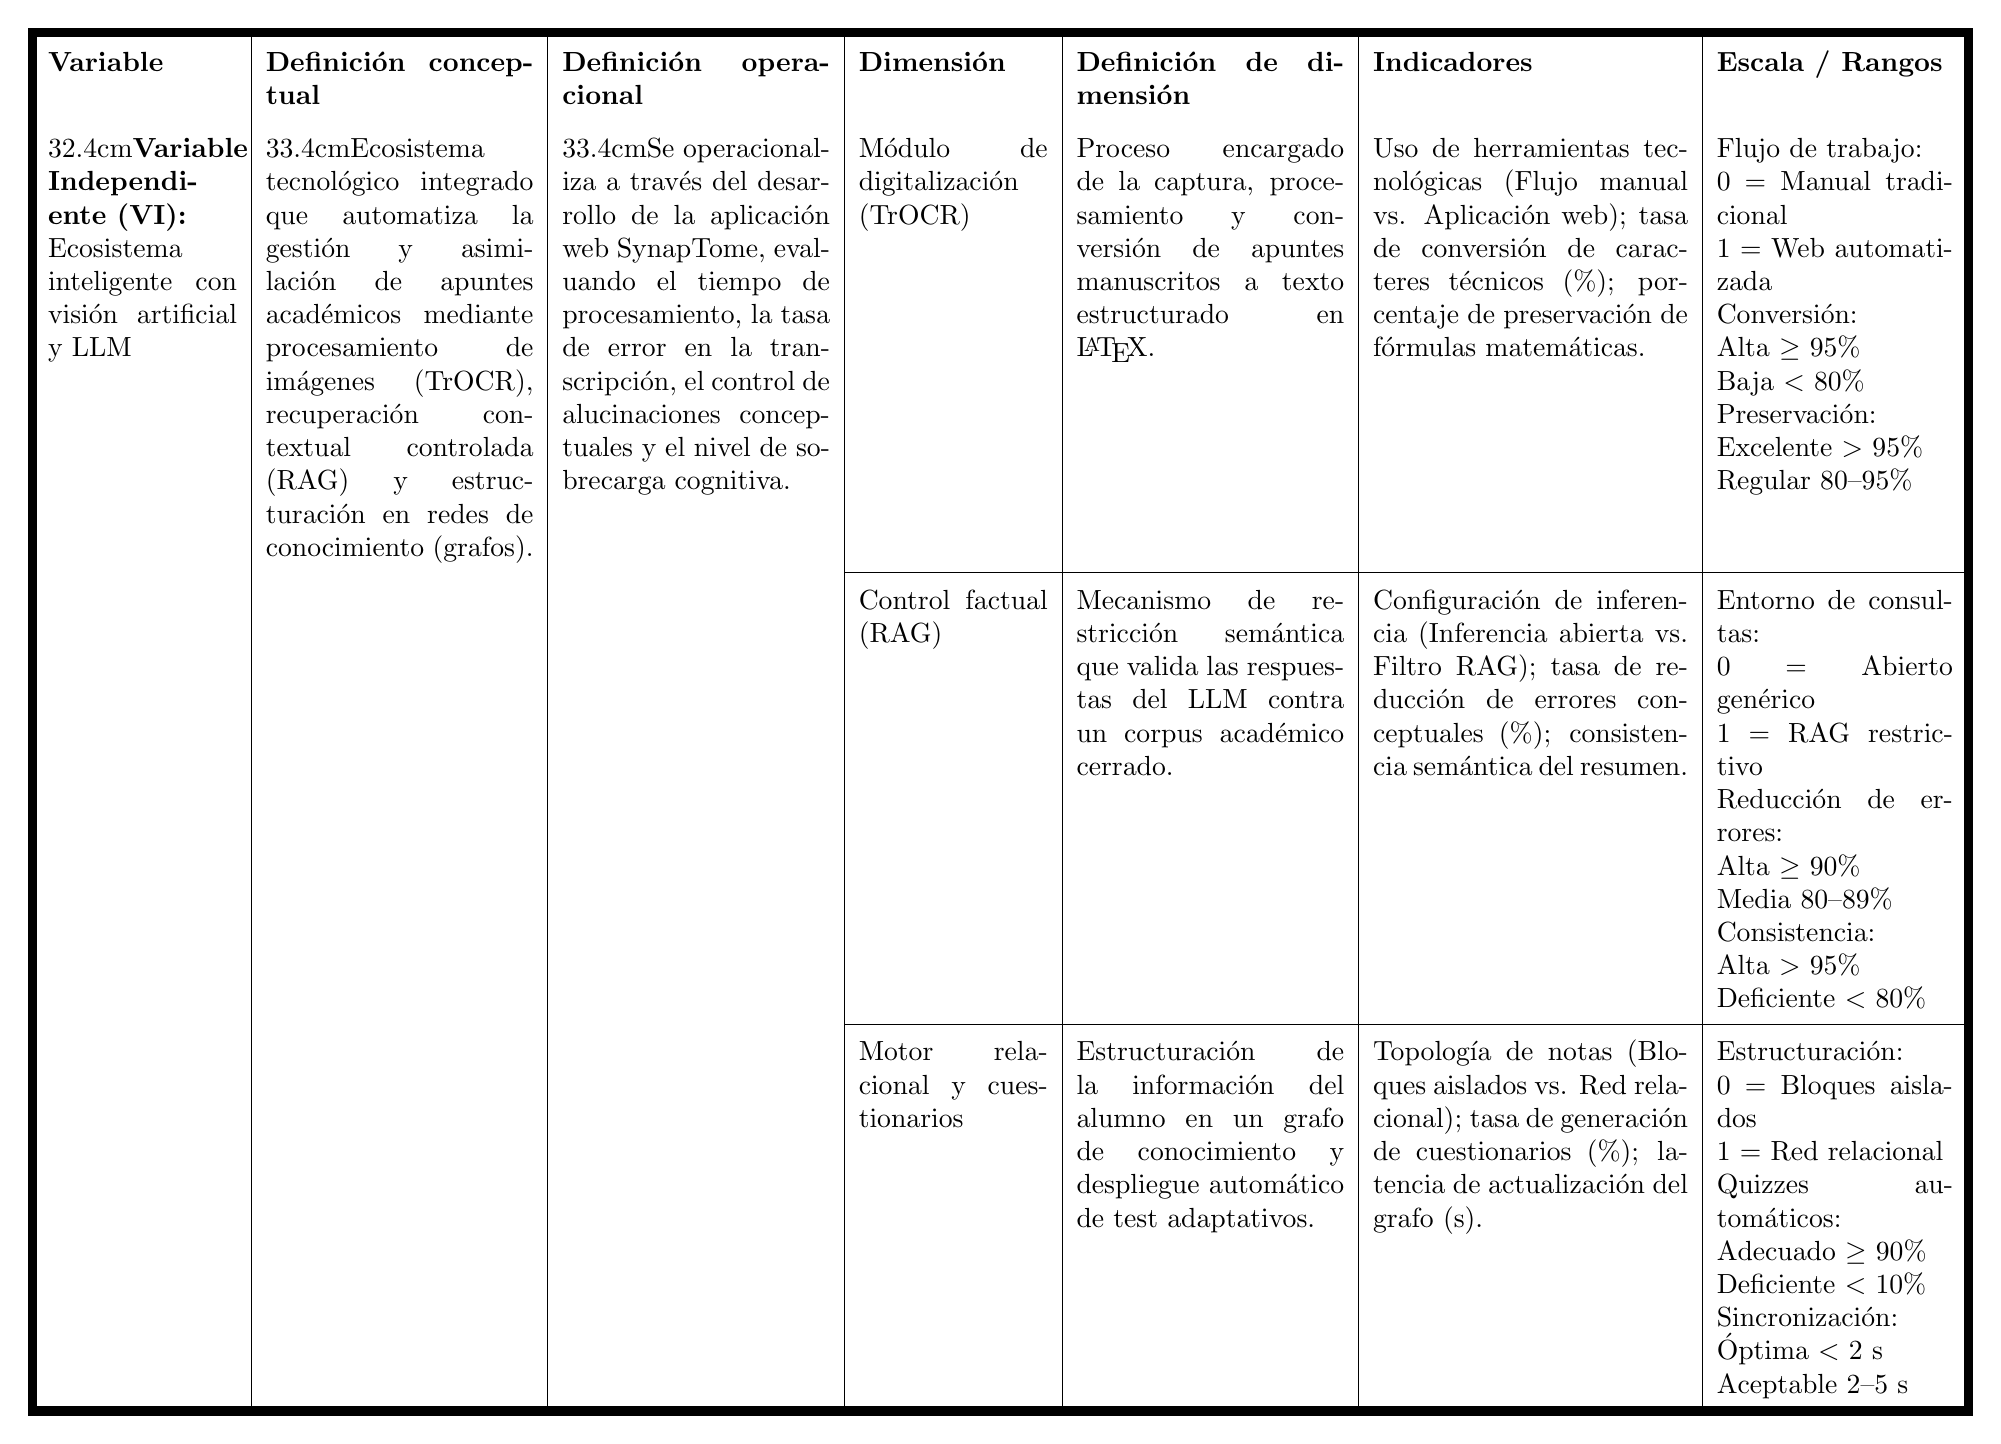
\begin{tikzpicture}
\node[inner sep=0pt] (table) {
\begin{tabular}{|p{2.4cm}|p{3.4cm}|p{3.4cm}|p{2.4cm}|p{3.4cm}|p{4.0cm}|p{3.0cm}|}

\hline
\textbf{Variable} &
\textbf{Definición conceptual} &
\textbf{Definición operacional} &
\textbf{Dimensión} &
\textbf{Definición de dimensión} &
\textbf{Indicadores} &
\textbf{Escala / Rangos} \\
\thickhline

%====================================================
% VARIABLE INDEPENDIENTE
%====================================================
\multirow{3}{2.4cm}{\textbf{Variable Independiente (VI):} \newline Ecosistema inteligente con visión artificial y LLM}
&
\multirow{3}{3.4cm}{Ecosistema tecnológico integrado que automatiza la gestión y asimilación de apuntes académicos mediante procesamiento de imágenes (TrOCR), recuperación contextual controlada (RAG) y estructuración en redes de conocimiento (grafos).}
&
\multirow{3}{3.4cm}{Se operacionaliza a través del desarrollo de la aplicación web SynapTome, evaluando el tiempo de procesamiento, la tasa de error en la transcripción, el control de alucinaciones conceptuales y el nivel de sobrecarga cognitiva.}
&
Módulo de digitalización (TrOCR)
&
Proceso encargado de la captura, procesamiento y conversión de apuntes manuscritos a texto estructurado en \LaTeX{}.
&
Uso de herramientas tecnológicas (Flujo manual vs. Aplicación web); tasa de conversión de caracteres técnicos (\%); porcentaje de preservación de fórmulas matemáticas.
&
Flujo de trabajo: \newline 0 = Manual tradicional \newline 1 = Web automatizada \newline
Conversión: \newline Alta $\geq$ 95\% \newline Baja $<$ 80\% \newline
Preservación: \newline Excelente $>$ 95\% \newline Regular 80--95\%
\\
\cline{4-7}
& & &
Control factual (RAG)
&
Mecanismo de restricción semántica que valida las respuestas del LLM contra un corpus académico cerrado.
&
Configuración de inferencia (Inferencia abierta vs. Filtro RAG); tasa de reducción de errores conceptuales (\%); consistencia semántica del resumen.
&
Entorno de consultas: \newline 0 = Abierto genérico \newline 1 = RAG restrictivo \newline
Reducción de errores: \newline Alta $\geq$ 90\% \newline Media 80--89\% \newline
Consistencia: \newline Alta $>$ 95\% \newline Deficiente $<$ 80\%
\\
\cline{4-7}
& & &
Motor relacional y cuestionarios
&
Estructuración de la información del alumno en un grafo de conocimiento y despliegue automático de test adaptativos.
&
Topología de notas (Bloques aislados vs. Red relacional); tasa de generación de cuestionarios (\%); latencia de actualización del grafo (s).
&
Estructuración: \newline 0 = Bloques aislados \newline 1 = Red relacional \newline
Quizzes automáticos: \newline Adecuado $\geq$ 90\% \newline Deficiente $<$ 10\% \newline
Sincronización: \newline Óptima $<$ 2 s \newline Aceptable 2--5 s
\\
\hline

\end{tabular}
};

\draw[line width=3.5pt]
(table.north west) rectangle (table.south east);
\end{tikzpicture}%
}

\end{table}

\clearpage

%====================================================
% TABLA DE OPERACIONALIZACIÓN DE VARIABLE DEPENDIENTE
%====================================================
\begin{table}[htbp]
\centering
\scriptsize

\caption{Operacionalización de la Variable Dependiente (VD)}
\label{tab:operacionalizacion_vd}

\renewcommand{\arraystretch}{1.6}
\setlength{\tabcolsep}{5pt}

\resizebox{\linewidth}{!}{%
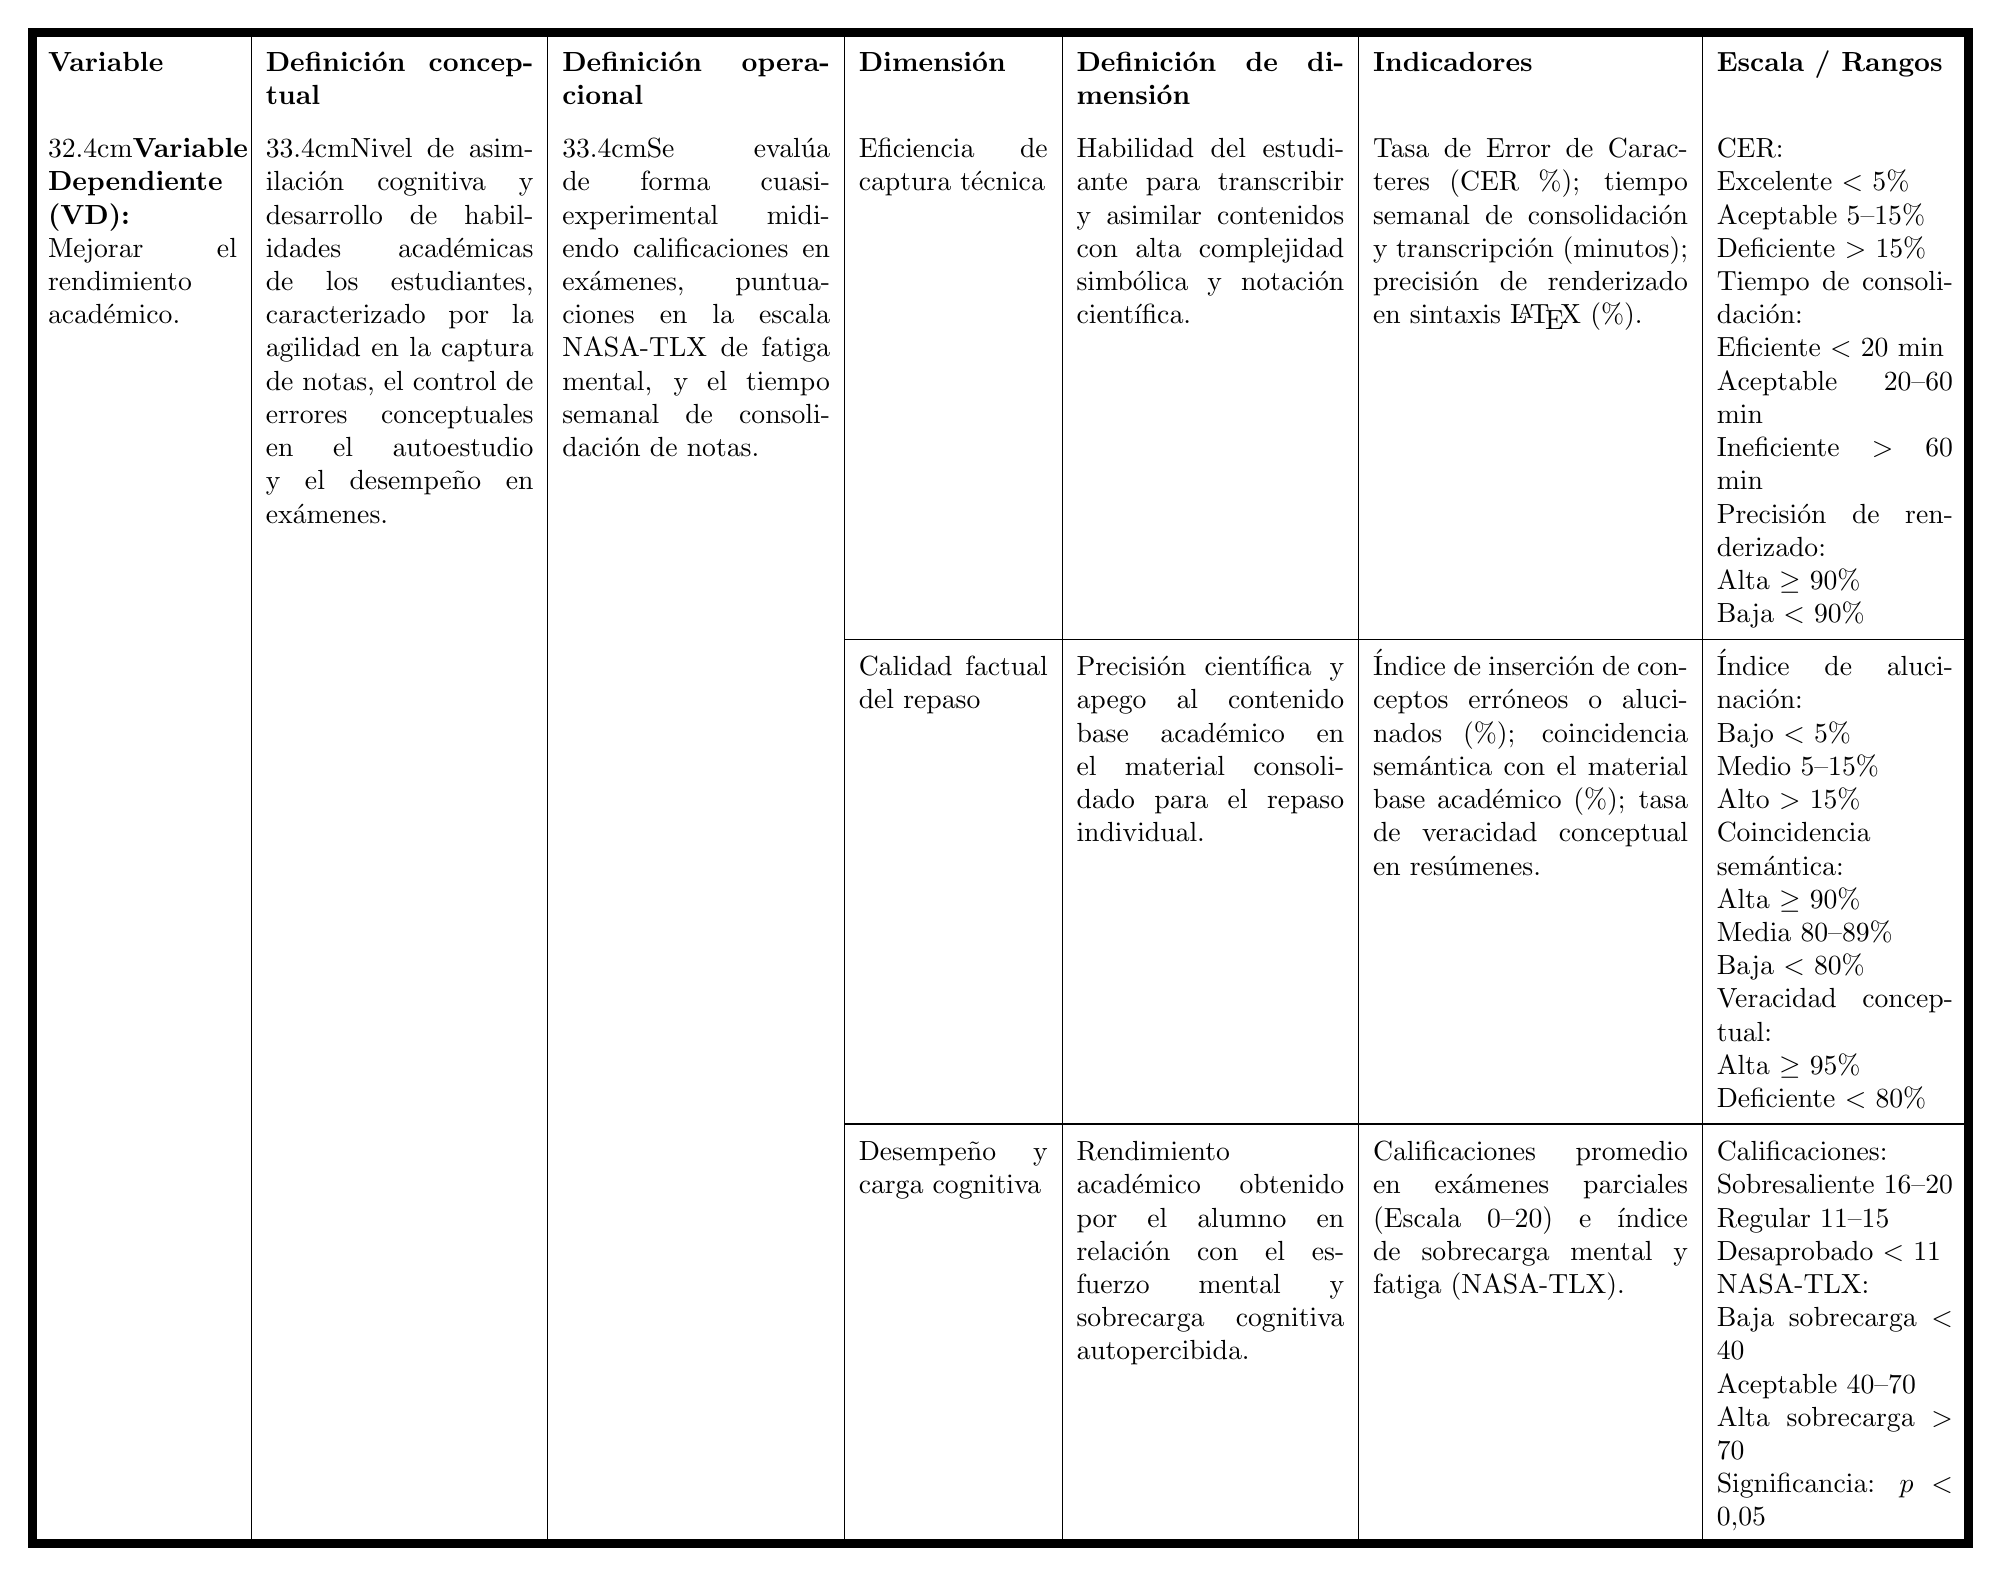
\begin{tikzpicture}
\node[inner sep=0pt] (table) {
\begin{tabular}{|p{2.4cm}|p{3.4cm}|p{3.4cm}|p{2.4cm}|p{3.4cm}|p{4.0cm}|p{3.0cm}|}

\hline
\textbf{Variable} &
\textbf{Definición conceptual} &
\textbf{Definición operacional} &
\textbf{Dimensión} &
\textbf{Definición de dimensión} &
\textbf{Indicadores} &
\textbf{Escala / Rangos} \\
\thickhline

%====================================================
% VARIABLE DEPENDIENTE
%====================================================
\multirow{3}{2.4cm}{\textbf{Variable Dependiente (VD):} \newline Mejorar el rendimiento académico.}
&
\multirow{3}{3.4cm}{Nivel de asimilación cognitiva y desarrollo de habilidades académicas de los estudiantes, caracterizado por la agilidad en la captura de notas, el control de errores conceptuales en el autoestudio y el desempeño en exámenes.}
&
\multirow{3}{3.4cm}{Se evalúa de forma cuasi-experimental midiendo calificaciones en exámenes, puntuaciones en la escala NASA-TLX de fatiga mental, y el tiempo semanal de consolidación de notas.}
&
Eficiencia de captura técnica
&
Habilidad del estudiante para transcribir y asimilar contenidos con alta complejidad simbólica y notación científica.
&
Tasa de Error de Caracteres (CER \%); tiempo semanal de consolidación y transcripción (minutos); precisión de renderizado en sintaxis \LaTeX{} (\%).
&
CER: \newline Excelente $<$ 5\% \newline Aceptable 5--15\% \newline Deficiente $>$ 15\% \newline
Tiempo de consolidación: \newline Eficiente $<$ 20 min \newline Aceptable 20--60 min \newline Ineficiente $>$ 60 min \newline
Precisión de renderizado: \newline Alta $\geq$ 90\% \newline Baja $<$ 90\%
\\
\cline{4-7}
& & &
Calidad factual del repaso
&
Precisión científica y apego al contenido base académico en el material consolidado para el repaso individual.
&
Índice de inserción de conceptos erróneos o alucinados (\%); coincidencia semántica con el material base académico (\%); tasa de veracidad conceptual en resúmenes.
&
Índice de alucinación: \newline Bajo $<$ 5\% \newline Medio 5--15\% \newline Alto $>$ 15\% \newline
Coincidencia semántica: \newline Alta $\geq$ 90\% \newline Media 80--89\% \newline Baja $<$ 80\% \newline
Veracidad conceptual: \newline Alta $\geq$ 95\% \newline Deficiente $<$ 80\%
\\
\cline{4-7}
& & &
Desempeño y carga cognitiva
&
Rendimiento académico obtenido por el alumno en relación con el esfuerzo mental y sobrecarga cognitiva autopercibida.
&
Calificaciones promedio en exámenes parciales (Escala 0--20) e índice de sobrecarga mental y fatiga (NASA-TLX).
&
Calificaciones: \newline Sobresaliente 16--20 \newline Regular 11--15 \newline Desaprobado $<$ 11 \newline
NASA-TLX: \newline Baja sobrecarga $<$ 40 \newline Aceptable 40--70 \newline Alta sobrecarga $>$ 70 \newline
Significancia: $p < 0{,}05$
\\
\hline

\end{tabular}
};

\draw[line width=3.5pt]
(table.north west) rectangle (table.south east);
\end{tikzpicture}%
}

\end{table}

\end{landscape}